\documentclass[a4,12pt]{article}

\usepackage[utf8]{inputenc}
\usepackage[spanish]{babel}
\usepackage[margin=1.5cm]{geometry}
\usepackage{graphicx}
\usepackage{color}
\usepackage{import}
\usepackage{float }
\usepackage{mathtools}


\usepackage{hyperref}

\parindent 0em

%\usepackage{times}
\renewcommand{\familydefault}{\sfdefault}

\title{Resolución de problemas con GNU OCTAVE}
\author{Lamya Hafs}
%\date{}

\begin{document}

\maketitle
\bigskip
\bigskip
\bigskip
\begin{figure}[H]
  \centering
    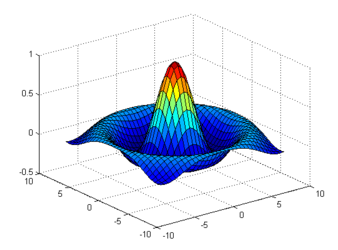
\includegraphics{imagenes/octave}
\end{figure}
\newpage

\maketitle

\begin{abstract}
El documento explica como se ha conseguido resolver problemas mediante el software GNU Octav.\\ Los problemas a resolver son:\\
- Problema de programacion lineal denominado "El problema de dieta".\\
- Ilustración gráfica del tiempo de ejecución del algoritmo de ordenamiento rápido "Quicksort" con diferentes tamaños de entrada.\\

\end{abstract}

\tableofcontents
\newpage

\section{Problema de dieta}

\subsection{Descripción del problema}
Se desea añadir a la dieta de ciertos animales de granja cantidades extra de tiamina, fósforo y hierro.\\
Para ello en el mercado existen dos preparados en polvo diferentes: Fosfatón y Ferroforo. Estos
contienen los nutrientes en las cantidades que se indican a continuación. Cada onza de Ferroforo
contiene 0.15 mg de tiamina, 0.75 mg de fósforo y 1.30 mg de hierro. Cada onza de Fosfatón contiene 0.10 mg de tiamina, 1.70 mg de fósforo y 1.10 mg de hierro. Deseamos que cada animal reciba al día, al menos 1.00 mg de tiamina, 7.50 mg de fósforo y 10.00 mg de hierro.\\
El costo de cada onza de Ferroforo es de 0.02 euros y el de Fosfatón es de $\frac{5}{3}$ de céntimo de euro poronza. Determinar las cantidades de Ferroforo y Fosfatón que debemos suministrar a cada animal de forma que el costo de este suplemento a la dieta sea mínimo.\\

\subsection{Solución}
En primer lugar expresamos los datos del problema en forma de tabla, lo que nos dará una mejor
perspectiva de los mismos:\\

\begin{center}
\begin{tabular}{|c|c|c|c|c|} \hline
\textbf{}   &  \textbf{Tiamina}  &  \textbf{Fósforo} &  \textbf{Hierro}  &  \textbf{Coste de los igredientes} \\ \hline
Ferroforo  & 0.15 mg/oz  &  0.75 mg/oz & 1.30 mg/oz  &  2 ct/oz  \\  \hline
Fosfatón  & 0.10 mg/oz  &  1.70 mg/oz & 1.10 mg/oz  &  $\frac{5}{3}$ ct/oz  \\  \hline
\end{tabular}
\end{center}

• Definición de las variables del problema:\\
Sean $x_1$ y $x_2$ las cantidades, en onzas, de Ferroforo y Fosfatón, respectivamente, que debemos añadir a la dieta de los animales diariamente.\\
• Restricciones del problema:\\
Al echar a la dieta $x_1$ onzas de Ferroforo y $x_2$ onzas de Fosfatón estaríamos proporcionando a la misma el siguiente aporte nutricional diario:\\

\begin{center}
                  0.15 $x_1$ + 0.10 $x_2$ mg de Tiamina\\
                  0.75 $x_1$ + 1.70 $x_2$ mg de Fósforo\\
                  1.30 $x_1$ + 1.10 $x_2$ mg de Hierro\\
\end{center}
                  
Como deseamos que cada animal reciba al día, al menos 1.00 mg de tiamina, 7.50 mg de fósforo y 10.00 mg de hierro. Deberemos imponer las siguientes restricciones:\\

\begin{center}
                  0.15 $x_1$ + 0.10 $x_2\ge 1.00$  \\
                  0.75 $x_1$ + 1.70 $x_2\ge 7.50$  \\
                  1.30 $x_1$ + 1.10 $x_2\ge 10.00$ \\
\end{center}
                  
• Restricciones de no negatividad:\\
Tal y como hemos definido las variables del problema no tiene ningún sentido que éstas tomen valores negativos. De manera que también impondremos las restricciones:\\

\begin{center}
         $x_1\ge 0$ \\
         $x_2\ge 0$ \\
\end{center}

Estas restricciones se suelen expresar de forma conjunta del siguiente modo:\\

\begin{center}
         $x_1 , x_2 \ge 0$\\
\end{center}

y se les llama las restricciones de no negatividad.\\

• Definición de la función que representa el objetivo que pretendemos alcanzar:\\
Es lógico pensar que habrá muchas pares de valores ($x_1$, $x_2$) que cumplirán todas las restricciones del problema. Cada uno de estos pares de valores ($x_1$,$x_2$), que significa echar, diariamente, a la dieta de los animales $x_1$ onzas de Ferroforo y $x_2$ onzas de Fosfatón, , tendrá un costo de 2 $x_1$ + $\frac{5}{3}x_2$  céntimos de euro.\\

Luego si llamamos z = 2 $x_1$ + $\frac{5}{3}x_2$  , z representa el costo, en céntimos de euro, asociado al par ($x_1$, $x_2$) de valores de las variables.\\

Es evidente que nuestro objetivo será determinar el par ($x_1$, $x_2$) que cumpliendo todas las restricciones del problema haga mínimo el valor de la función z.\\

Luego el problema que hemos de resolver lo podemos expresar del siguiente modo:\\

\begin{displaymath}
P = \left\{ \begin{array}{ll}
 min z=2x_{1}+\frac{5}{3}x_{2}\\
\text{sujeto a :}\\
   0.15x_{1}+0.10x_{2}  \geq 1.00\\
   0.75x_{1}+1.70x_{2}  \geq 7.50\\
   0.30x_{1}+1.10x_{2}  \geq  10.00\\
       x_{1} , x_{2}  \geq  0
\end{array}
\right.
\end{displaymath}

\subsection{Solución en OCTAVE}
 
\textbf {La introduccion de los dados del problema en OCTAVE: } apartir del resultado conseguido  tenemos que resolver tanto $x_1$ como $x_2$ para encontrar el coste minimo.\\
Para ello seguimos los pasos siguientes : \\

• Primero se introducen en Octave los factores de la primera parte de cada ecuación .\\
\begin{verbatim}
octave-3.2.4:1> a =[0.15,0.10;0.75,1.70;1.30,1.10]
a =

   0.15000   0.10000
   0.75000   1.70000
   1.30000   1.10000
   
\end{verbatim}

• Luego se introducen los factores de la segunda parte de cada ecuación.\\
\begin{verbatim}
octave-3.2.4:2> b=[1;7.5;10]
b =

    1.0000
    7.5000
   10.0000
   
\end{verbatim}

• los valores resueltos con Octave de $x_1$ y $x_2$ son :\\
\begin{verbatim}
octave-3.2.4:3> a\b
ans =

   6.2983
   1.6347
\end{verbatim}

\section{Problema de QuickSort}
\subsection{Descripción del problema}
\textbf {Ordenamiento Rápido (Quicksort): } es un algoritmo basado en la técnica de divide y vencerás, que permite, en promedio, ordenar n elementos en un tiempo proporcional a n log n.\\
Esta es la técnica de ordenamiento más rápida conocida.\\

\subsection{El algoritmo fundamental de QuickSort}
• Elegir un elemento de la lista de elementos a ordenar, al que llamaremos pivote.\\

• Resituar los demás elementos de la lista a cada lado del pivote, de manera que a un lado queden todos los menores que él, y al otro los mayores. En este momento, el pivote ocupa exactamente el lugar que le corresponderá en la lista ordenada.\\

• La lista queda separada en dos sublistas, una formada por los elementos a la izquierda del pivote, y otra por los elementos a su derecha.\\

• Repetir este proceso de forma recursiva para cada sublista mientras éstas contengan más de un elemento. Una vez terminado este proceso todos los elementos estarán ordenados. Como se puede suponer, la eficiencia del algoritmo depende de la posición en la que termine el pivote elegido.\\

• En el mejor caso, el pivote termina en el centro de la lista, dividiéndola en dos sublistas de igual tamaño. En este caso, el orden de complejidad del algoritmo es O(n·log n).\\

• En el peor caso, el pivote termina en un extremo de la lista. El orden de complejidad del algoritmo es entonces de 0($n^2$). El peor caso dependerá de la implementación del algoritmo, aunque habitualmente ocurre en listas que se encuentran ordenadas, o casi ordenadas.\\

• En el caso promedio, el orden es O(n·log n).\\

\subsection{Pasos de QuickSort}
\begin{figure}[H]
  \centering
    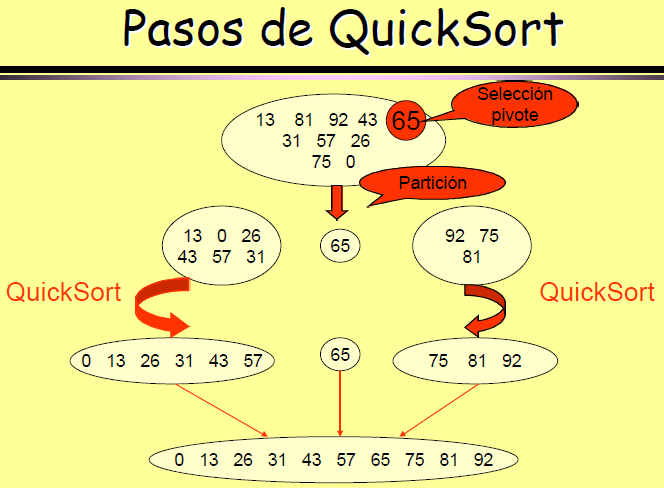
\includegraphics{imagenes/pasosQuickSort}
\end{figure}

\subsection{ilustración 2D en el peor caso de QuickSort en OCTAVE}
El peor caso como se ha explicado es cuando la complejidad igual a O($n^2$), el plot de ($n^2$) usando OCTAVE es seguir los siguientes pasos:\\
• Se introduce en Octave primero el intervalo de los numero que se quiere que se toma n, en el ejemplo propuesto toma los valores entre [0,10].\\

\begin{verbatim}
ctave:4> y=0:0.1:10;
octave:5> plot(y,pow2(y));
\end{verbatim}

• Luego se muestra graficamente el plot de ($n^2$).\\
\begin{verbatim}
octave:5> plot(y,pow2(y));
\end{verbatim}
\begin{figure}[H]
  \centering
    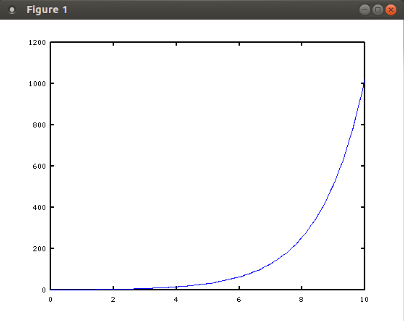
\includegraphics{imagenes/plot2}
\end{figure}

\subsection{ilustración 3D en el peor caso de QuickSort en OCTAVE}
\begin{verbatim}
octave:4> z=[0:0.1:10];
octave:5> plot3(z,pow2(z))
\end{verbatim}
\begin{figure}[H]
  \centering
    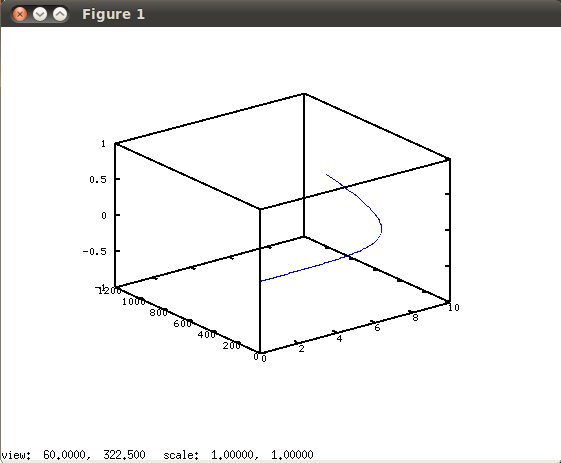
\includegraphics{imagenes/plot3}
\end{figure}

\end{document}

